\documentclass[a4paper,12pt]{report}
\usepackage[utf8]{inputenc}
\usepackage{graphicx}
\usepackage[margin=1in]{geometry}
\usepackage{setspace}
\usepackage{amsmath}
\usepackage{caption}
\usepackage{subcaption}
%\usepackage{titlesec}

\begin{document}
\setcounter{chapter}{3}
\chapter{Simulating flow in a Lid Driven Cavity using OpenFOAM}
\flushleft In this chapter we would learn how to solve a lid driven cavity problem using icoFoam solver and viewing the results in ParaView. As you might recollect from the 2nd chapter we, learned how to create the case file in OpenFoam and write its blockMeshDict file.
\flushleft You may review the previous chapter to see the problem statement for a lid driven cavity. Here in this problem we have a rectangular box of unit thickness with top surface moving with a velocity of 1 m/s and the other three sides fixed, as shown in fig \ref{geometry}$:$ 
\flushleft Here we have considered a Re of 100.

\begin{figure}[ht]  
\begin{center}  
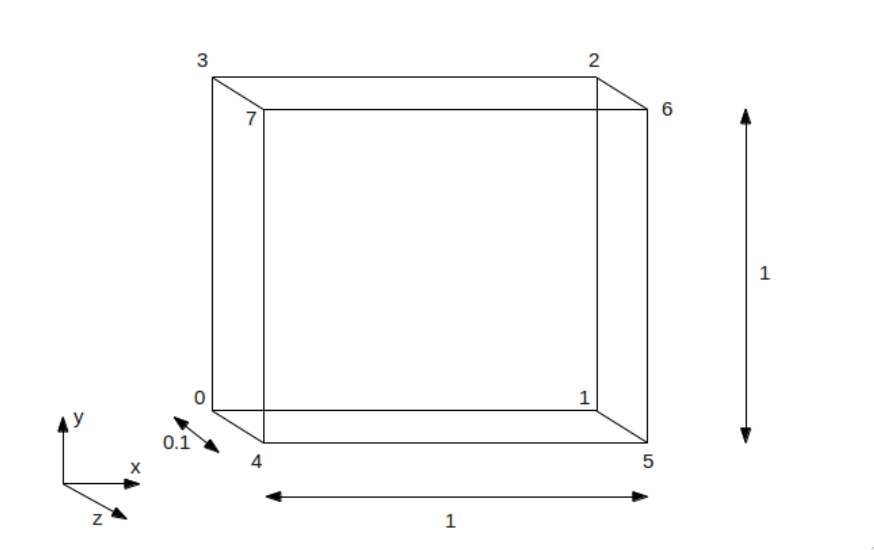
\includegraphics[scale=0.4]{geometry.png}
\caption{Geomtery of 2-D lid driven cavity}
\label{geometry}
\end{center}  
\end{figure}

\flushleft Now to solve our present problem open acommand terminal by pressing $<$ctrl$>$, $<$Alt$>$ and $<$T$>$ simulataneously. After this enter the path for the current case file as shown below$:$
\flushleft cd run/tutorial/incompressible/icoFoam/cavity
\flushleft After openning the required case file enter 'ls'. This would show the folders within this case file. Here as mentioned in chapter 2 you would find three folders by the name$:$

\begin{itemize}
  \item 0
  \item constant
  \item system
\end{itemize}

\flushleft Now if you press 'cd 0' <enter> and then 'ls' <enter> in the command terminal, you would find two folders given as$:$

\begin{itemize}
  \item P
  \item U
\end{itemize}

\flushleft These folders gives the initial boundary conditions for pressure (i.e. P), velocity (i.e. U), temperature, etc of the geomtery. After this go back to the cavity folder by typing 'cd ..' $<$enter$>$.
\flushleft Now if you open the constant folder by entering 'cd constant' <enter> in the command terminal followed by 'ls' <enter> you would find two folder$:$

\begin{itemize}
  \item polyMesh
  \item transportProperties
\end{itemize}

\flushleft Here polyMesh folder contains the blockMeshDict file. You can open this by typing 'cd poymesh' $<$enter$>$ followed by 'ls' $<$enter$>$ in the command terminal and then type 'gedit blockMeshDict'. This would show you the blockMeshDict file in text editor which contains the veritces, blocks and boundary patches of the geometry. The tranportProperties contain properties of the fluid medium used in this this problem. 
\flushleft Now you can go back to the cavity folder by entering cd .. twice in the command terminal. After this type 'cd system' <enter> followed by 'ls' $<$enter$>$. This would show you the three folders within system file.
\begin{itemize}
  \item ControlDict
  \item fvSchemes
  \item fvSolution
\end{itemize}

\flushleft Here controlDict file contains control parameters for start and stop of the number of iterations, fvSolution contain discretization schemes used for simualtion of this problem and fvSchemes contains equations for solver, tolerance, etc.
\flushleft To mesh the geometry go back to the cavity folder in the command terminal and enter the following and press $<$enter$>$:
\flushleft blockMesh
\flushleft This would mesh the geometry as shown in the fig \ref{blockmesh}$:$

\begin{figure}[ht]  
\begin{center}  
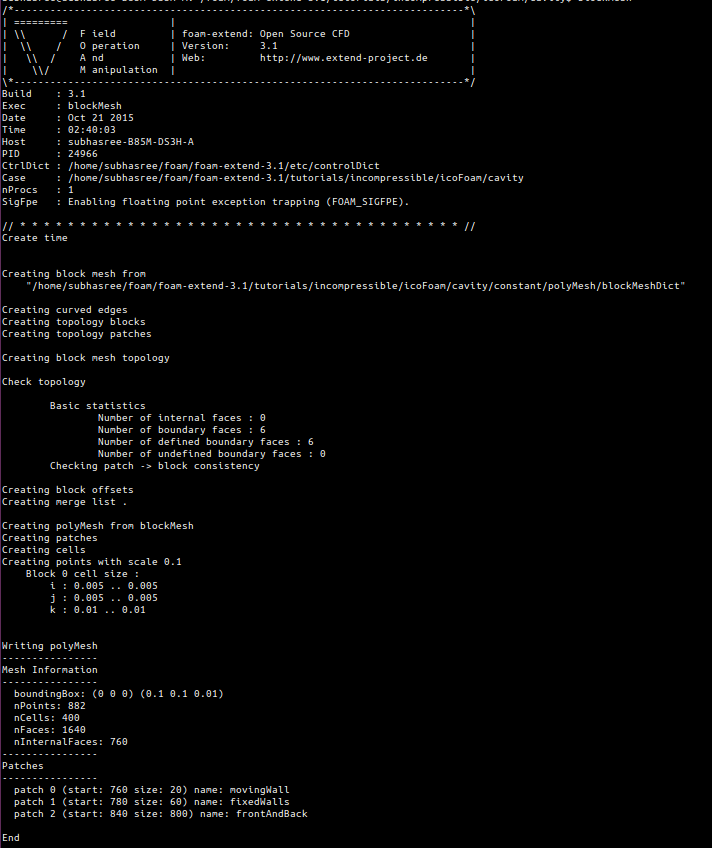
\includegraphics[scale=0.7]{blockMesh.png}
\caption{Meshing of the 2-D geometry in OpenFOAM}
\label{blockmesh}
\end{center}  
\end{figure}

\flushleft As you can see, we have used course mesh for this problem. If there are some error in the blockMesDict file, it would be shown in the command terminal. You can also type 'checkMesh' $<$enter$>$ in the command terminal to check the different properties of the meshed geometry like number of cells, skewness, etc. 
\flushleft After this to view the meshed geometry, you can type 'paraFoam' $<$enter$>$ in the command terminal. This woould open the ParaView window. Now on the ParaView window press apply on the left hand side of the Object Inspector Menu to view the meshed geometry, as shown in fig \ref{paraview1}. After inspecting the geomety you may close the ParaView window and switch back to the command terminal.

\begin{figure}[ht]  
\begin{center}  
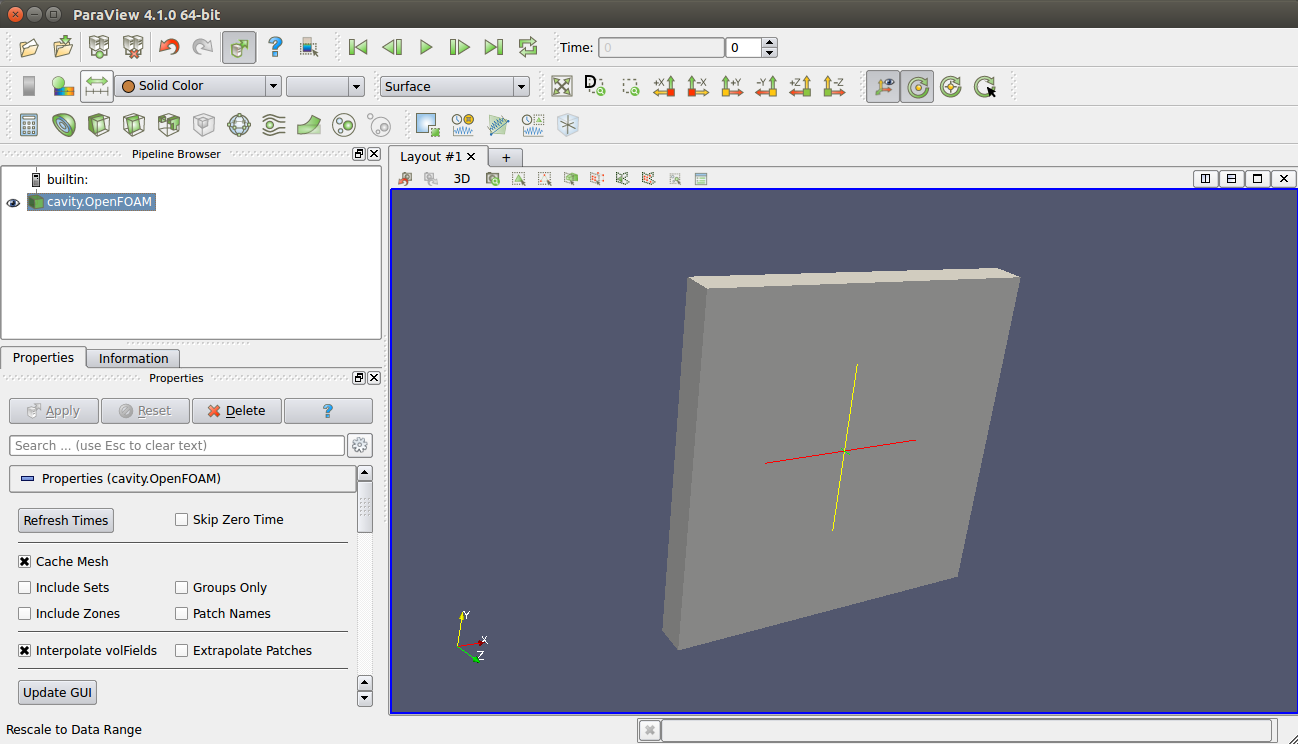
\includegraphics[scale=0.32]{paraview1.png}
\caption{Visualization of the 2-D geometry in ParaView}
\label{paraview1}
\end{center}  
\end{figure}

\flushleft Now for simulating this particular problem we have used icoFoam solver. This is a Transient solver for incompressible, laminar flow of Newtonian fluids. To solve this problem type 'icoFoam' <enter> in the command terminal. You can see the progressing iterations in the terminal window along with the residual values. After it ends type 'paraFoam' $<$enter$>$ in the terminal window for post-processing. 
\flushleft This would open the ParaView window. As mentioned previously press apply on the left hand side of the Object Inspector Menu to view the new geometry. After this you can check or uncheck the different regions within the mesh region in  the Object Inspector Menu to visualize differnt regions on the geomtery. Now to check the velocity contours select U from the drop-down Active Variable Control Menu, from the visible toolbar. This will show the initial velocity countour of the cavity, as shown in fig \ref{vel1}. Along with this you may also select the Toggle Colour Legend from the toolbar to visualize the legend.

\begin{figure}[ht]  
\begin{center}  
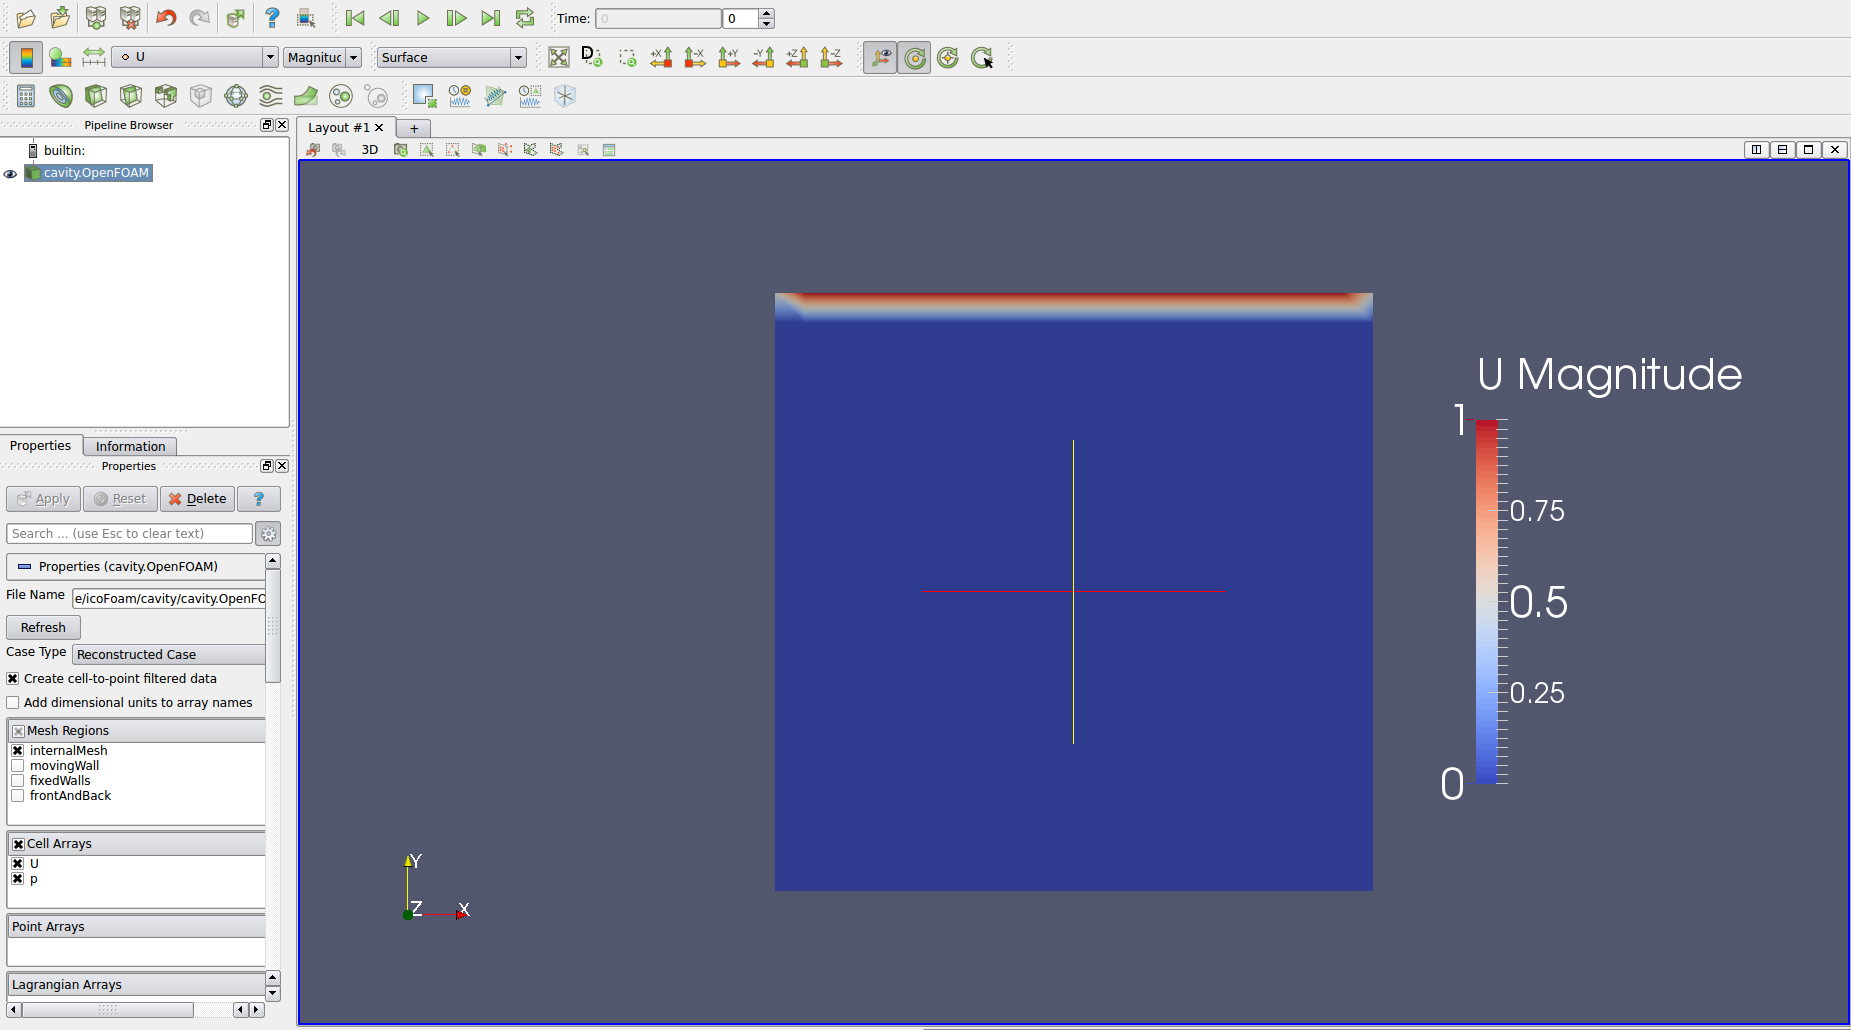
\includegraphics[scale=0.24]{vel1.png}
\caption{Velocity contour in the 2-D geometry at time 0 sec in ParaView}
\label{vel1}
\end{center}  
\end{figure}

\flushleft Now in the paraView window press the 'play' buttom from the VCR control. This would visualize the changing velocity countour along with the progressing iterations. You can see the final velocity contour as shown in fig \ref{vel2}.

\begin{figure}[ht]  
\begin{center}  
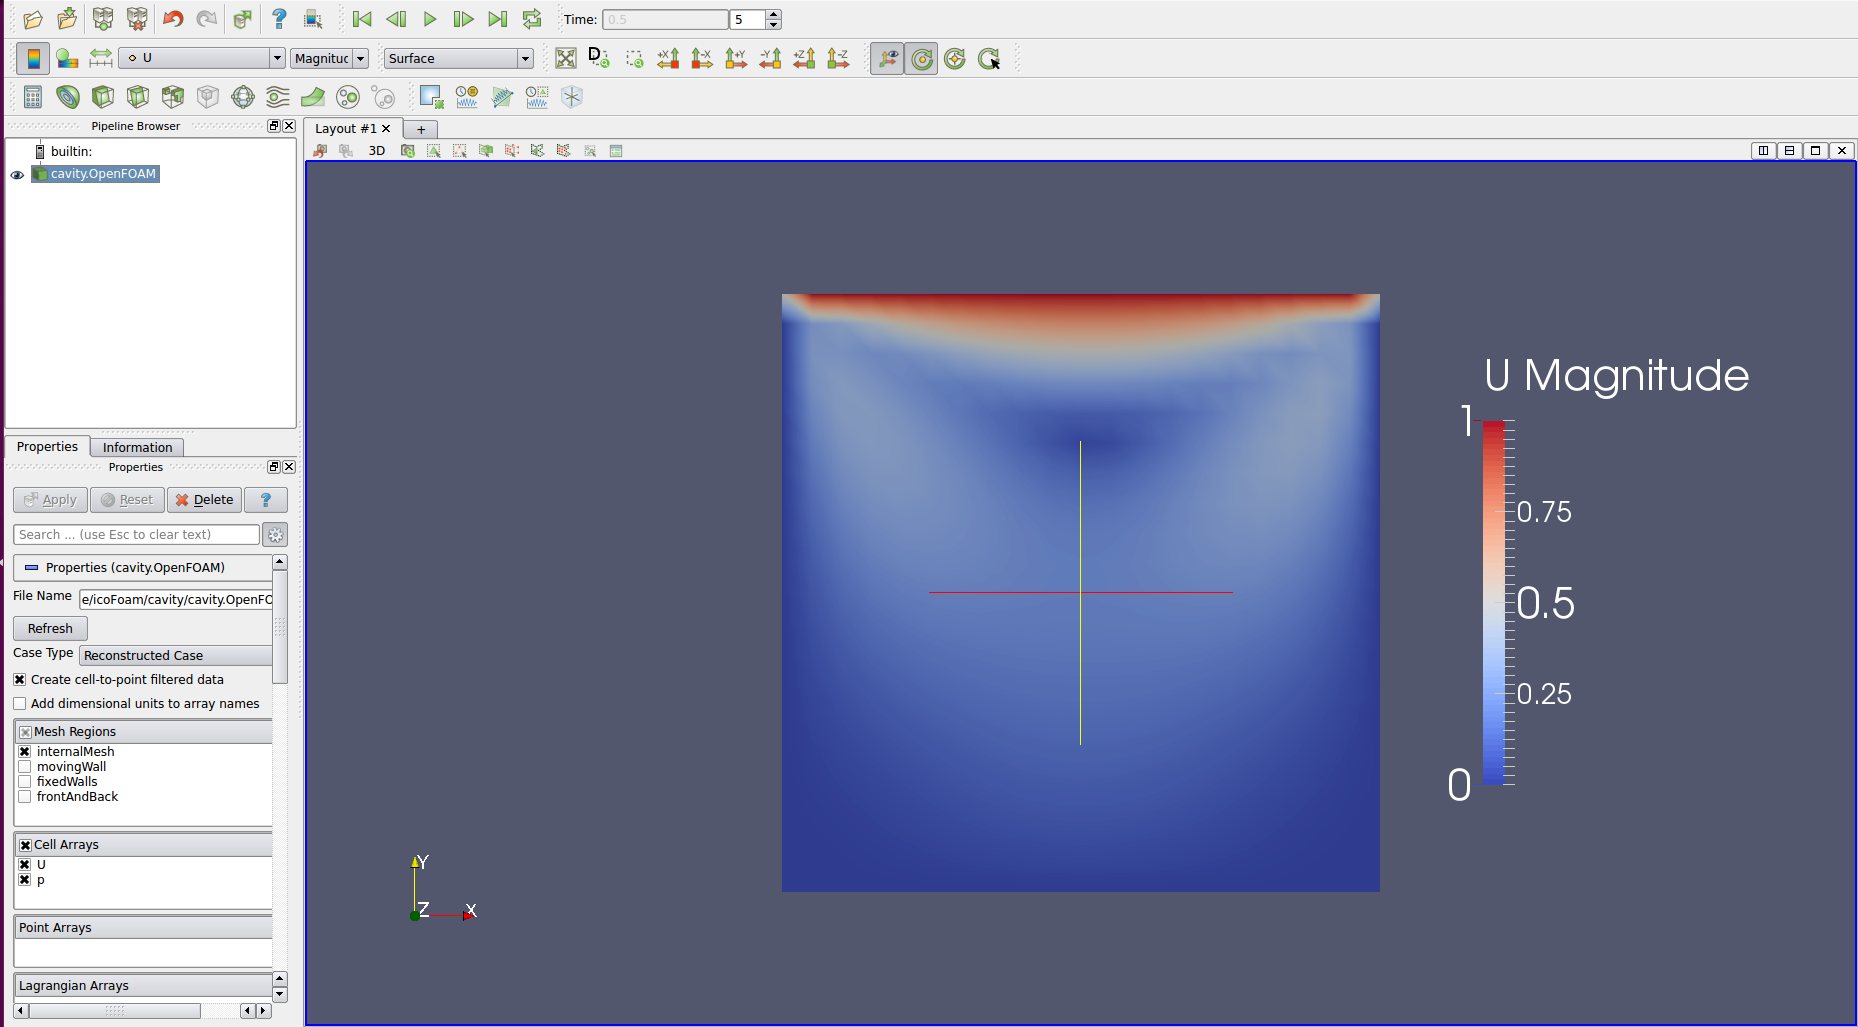
\includegraphics[scale=0.24]{vel2.png}
\caption{Velocity contour in the 2-D geometry at final state in ParaView}
\label{vel2}
\end{center}  
\end{figure}

\flushleft Now to validate our result we need to plot the u and v velocity in the domain. To do this click on the 'plot over line' object from the  Active Variable Control Menu bar. Now for our validation we need to plot u/U versus l/L in the X and Y axis. To do this select X-axis on the left hand side  Object Inspector Menu. This will show you the Pressure and velocity plot along X-direction.

\begin{figure}[ht]  
\begin{center}  
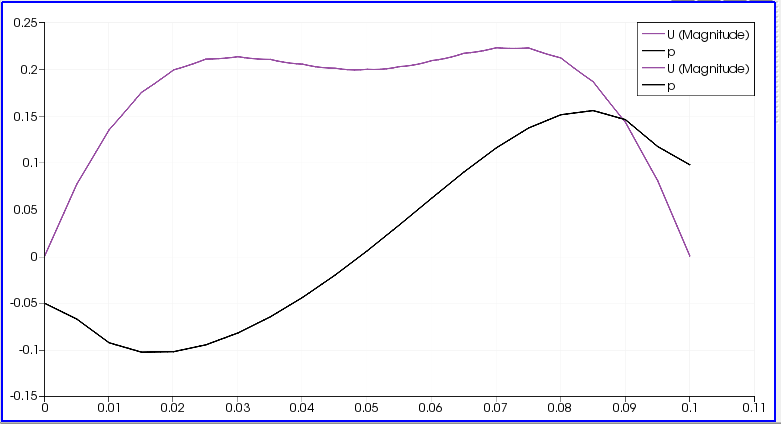
\includegraphics[scale=0.24]{xaxisvel.png}
\caption{Velocity contour in the 2-D geometry at final state in ParaView}
\label{xaxisvel}
\end{center}  
\end{figure}

\flushleft On selecting the Yaxis you will see the velocity along Y-axis.

\begin{figure}[ht]  
\begin{center}  
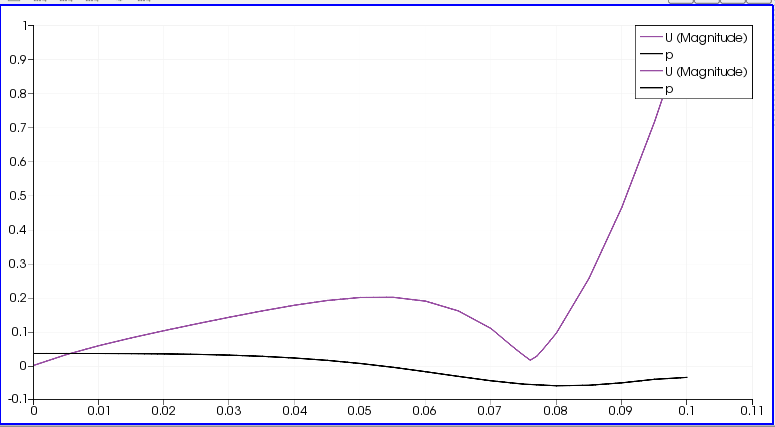
\includegraphics[scale=0.24]{yaxisvel.png}
\caption{Velocity contour in the 2-D geometry at final state in ParaView}
\label{yaxisvel}
\end{center}  
\end{figure}

\flushleft Now you may save these data by selecting File>Save As> and then give appropriate file name. These data will be saved in .csv format. After this open this file from home folder in libreoffice sheet. In the office sheet you can copy paste U:0 and P:1 on a new sheet and calculate it as U:0/U and P:1/L. And them plot them using chart utility. This would give you the following result.


\end{document}
